\documentclass[12pt,a4paper]{article}

% ─── Pachete ───
\usepackage[T1]{fontenc}
\usepackage[utf8]{inputenc}
\usepackage[romanian]{babel}
\usepackage{geometry}
\geometry{margin=2.5cm}
\usepackage{graphicx}
\usepackage{booktabs}
\usepackage{amsmath}
\usepackage{amssymb}
\usepackage{hyperref}
\usepackage{listings}
\usepackage{xcolor}
\usepackage{float}
\usepackage{enumitem}
\usepackage{caption}
\usepackage{subcaption}
\usepackage{tikz}
\usepackage{placeins}
\usetikzlibrary{arrows.meta, positioning, shapes.geometric}

% ─── Stil cod ───
\lstset{
    language=Python,
    basicstyle=\ttfamily\small,
    keywordstyle=\color{blue}\bfseries,
    stringstyle=\color{red!70!black},
    commentstyle=\color{green!50!black}\itshape,
    numbers=left,
    numberstyle=\tiny\color{gray},
    frame=single,
    breaklines=true,
    captionpos=b,
    showstringspaces=false,
    extendedchars=true,
    literate=
        {ă}{{\u{a}}}1 {Ă}{{\u{A}}}1
        {â}{{\^{a}}}1 {Â}{{\^{A}}}1
        {î}{{\^{i}}}1 {Î}{{\^{I}}}1
        {ș}{{\textcommabelow{s}}}1 {Ș}{{\textcommabelow{S}}}1
        {ț}{{\textcommabelow{t}}}1 {Ț}{{\textcommabelow{T}}}1
        {ş}{{\c{s}}}1 {Ş}{{\c{S}}}1
        {ţ}{{\c{t}}}1 {Ţ}{{\c{T}}}1,
}

% ─── Hyperref ───
\hypersetup{
    colorlinks=true,
    linkcolor=blue!70!black,
    citecolor=blue!70!black,
    urlcolor=blue!70!black,
}

\title{
    \textbf{Musicon} \\[0.5em]
    \large Generarea de playlist-uri Spotify bazate pe mood \\
    folosind Machine Learning și Reinforcement Learning
}
\author{
    \textbf{Badescu Bianca-Mădălina} \\[0.3em]
    \small Universitatea de Vest din Timișoara \\[0.1em]
    \small Facultatea de Informatică \\[0.3em]
    \small \textit{Disciplina: Inteligență Artificială}
}
\date{\today}

\begin{document}

\maketitle
\thispagestyle{empty}
\newpage

% ─── Cuprins ───
\tableofcontents
\newpage

% ═══════════════════════════════════════════════════════════════════
\section{Introducere}
% ═══════════════════════════════════════════════════════════════════

Platformele de streaming precum Spotify oferă acces la milioane de piese, dar descoperirea muzicii relevante pentru starea emoțională curentă a utilizatorului rămâne o problemă semnificativă. Sistemele de recomandare actuale se bazează pe istoricul de ascultare și pe filtrarea colaborativă și nu ia în considerare ce sentimente transmit melodiile și cum se pot corela acestea într-un playlist.

Proiectul \textbf{Musicon} abordează această problemă prin dezvoltarea unui sistem de generare automată a playlist-urilor bazat pe identificarea stării emoționale. Sistemul combină două paradigme fundamentale ale Inteligenței Artificiale:
\begin{itemize}
    \item \textbf{Machine Learning} (învățare supervizată) pentru clasificarea pieselor în funcție de mood, folosind caracteristici audio extrase din Spotify;
    \item \textbf{Reinforcement Learning} (învățare prin recompensă) pentru optimizarea selecției secvențiale a pieselor în playlist.
\end{itemize}

\textbf{Obiectivele principale ale proiectului:}
\begin{enumerate}
    \item Construirea unui dataset potrivit prin utilizarea a 10.000 de piese populare etichetate cu 8 stări emoționale diversificate.
    \item Antrenarea și compararea a 3 clasificatori ML (Decision Tree, Random Forest, K-Nearest Neighbors) pentru predicția mood-ului pe baza feature-urilor audio Spotify.
    \item Implementarea unui agent Q-Learning care modelează selecția pieselor ca un proces decizional Markovian (MDP) cu 192 de stări și 10 acțiuni.
    \item Dezvoltarea unei interfețe web interactive folosind Streamlit, care permite utilizatorilor să selecteze un mood prin 24 de preset-uri sau prin text liber.
\end{enumerate}


% ═══════════════════════════════════════════════════════════════════
\section{State of the Art}
% ═══════════════════════════════════════════════════════════════════

\subsection{Modelul circumplex al afectului}

Fundamentul teoretic al mapării emoționale în Musicon este \textbf{Modelul Circumplex al Afectului}, propus de James A. Russell în 1980 \cite{russell1980}. Acest model reprezintă stările emoționale ca puncte într-un spațiu bidimensional, având ca axe \textbf{valența} (plăcut -- neplăcut) și \textbf{activarea} (energie scăzută -- energie ridicată).

În contextul muzical, valența corespunde caracterului pozitiv sau negativ al unei piese (măsurat prin feature-ul Spotify \textit{valence}), iar activarea corespunde intensității perceptuale (măsurată prin \textit{energy}).

\subsection{Clasificarea emoțiilor în muzică}

Thayer \cite{thayer1989} a propus un model de clasificare în 4 cadrane bazat pe Modelul Circumplex al Afectului propus de Russell:
\begin{itemize}
    \item \textbf{Energie ridicată, valență pozitivă} -- Exuberant, entuziast
    \item \textbf{Energie ridicată, valență negativă} -- Anxios, furios
    \item \textbf{Energie scăzută, valență pozitivă} -- Calm, relaxat
    \item \textbf{Energie scăzută, valență negativă} -- Melancolic, trist
\end{itemize}

Musicon extinde această clasificare la \textbf{8 stări emoționale}, oferind o arie mai extinsă de stări: \textit{melancholic, dark, calm, nostalgic, romantic, happy, euphoric, energetic}.

\subsection{Sisteme de recomandare muzicală}

Sistemele de recomandare muzicală se împart în 3 categorii principale \cite{aggarwal2016}:
\begin{enumerate}
    \item \textbf{Filtrare colaborativă} -- recomandă piese ascultate de utilizatori similari (Last.fm, Pandora);
    \item \textbf{Filtrare bazată pe conținut} -- utilizează caracteristici audio pentru a găsi piese similare;
    \item \textbf{Abordări hibride} -- combină cele două metode.
\end{enumerate}

Musicon adoptă o abordare bazată pe conținut, folosind feature-uri audio Spotify și tehnici de ML/RL.

\subsection{Analiza sistemelor existente}

\subsubsection{Moodify (Sabriweiss, 2026)}

\textbf{Moodify} \cite{moodify2026} este un sistem hibrid de recomandare muzicală dezvoltat în Python cu Streamlit \cite{streamlit}, care combină procesarea limbajului natural (NLP), învățarea nesupervizată și filtrarea bazată pe conținut. Principalele caracteristici:

\begin{itemize}
    \item \textbf{Detecție mood:} 4 mood-uri (Happy, Sad, Calm, Energetic) prin selecție directă sau clasificare NLP cu \textbf{Logistic Regression} pe text liber (CountVectorizer)
    \item \textbf{Clasificare:} Algoritm \textit{rule-based} pe feature-uri audio (valence, energy, tempo) și \textbf{K-Means Clustering} cu 8 clustere
    \item \textbf{Recomandare:} Filtrare bazată pe conținut folosind \textbf{Euclidean distance} între profilul utilizatorului și piesele din dataset
    \item \textbf{Personalizare:} Construirea unui profil de gust pe baza pieselor salvate de utilizator
    \item \textbf{Feature-uri:} 6 feature-uri audio Spotify (energy, valence, tempo, danceability, acousticness, instrumentalness)
\end{itemize}

\subsubsection{Moodify (Orzanai, 2023)}

O altă variantă Moodify \cite{moodify2023} utilizează modelul \textbf{LightGBM} pentru clasificarea emoțiilor pieselor și cosine similarity pentru recomandare. Se bazează pe \textbf{modelul Thayer} cu 4 emoții (happiness, sadness, calmness, energy) și folosește un dataset construit prin principiul ``Wisdom of Crowds'' din playlist-uri Spotify. Alte implementări similare includ varianta Moodify de pe Devpost \cite{moodify2024devpost} și extensia Chrome Moodify AI \cite{moodify2024chrome}, ambele axate pe generarea de playlist-uri bazate pe mood.

\subsubsection{Comparație cu Musicon}

\begin{table}[H]
\centering
\caption{Comparație Musicon cu sisteme existente}
\label{tab:comparison}
\small
\begin{tabular}{lccc}
\toprule
\textbf{Caracteristică} & \textbf{Musicon} & \textbf{Moodify} & \textbf{Moodify} \\
 & & \scriptsize{(Sabriweiss)} & \scriptsize{(Orzanai)} \\
\midrule
Mood-uri              & 8   & 4             & 4      \\
Clasificator ML       & DT/RF/KNN & LogReg+KMeans & LightGBM \\
Reinforcement Learning & Da (Q-Learning) & Nu    & Nu     \\
Metrică similaritate  & Cosine        & Euclidean     & Cosine   \\
Feature-uri audio     & 8   & 6             & 8         \\
Personalizare Spotify & Da  & Parțial       & Nu        \\
Interfață             & Streamlit     & Streamlit     & Streamlit \\
Preset-uri mood       & 24  & 4             & --        \\
\bottomrule
\end{tabular}
\end{table}

\textbf{Caracteristici cheie ale Musicon:}
\begin{enumerate}
    \item \textbf{Clasificare extinsă (8 mood-uri)} -- față de cele 4 mood-uri standard din Thayer
    \item \textbf{Reinforcement Learning} -- singurul sistem care folosește Q-Learning pentru optimizarea secvențială a playlist-ului;
    \item \textbf{Compară 3 clasificatori ML} -- evaluare sistematică a Decision Tree, Random Forest și KNN
    \item \textbf{Integrare Spotify} -- fuziunea profilului utilizatorului cu cel al preset-ului pentru recomandări personalizate
\end{enumerate}

\FloatBarrier

% ═══════════════════════════════════════════════════════════════════
\section{Arhitectura Aplicației}
% ═══════════════════════════════════════════════════════════════════

Aplicația urmează o arhitectură modulară cu un flux secvențial clar (Figura \ref{fig:arhitectura}).

\begin{figure}[H]
\centering
\resizebox{0.95\textwidth}{!}{%
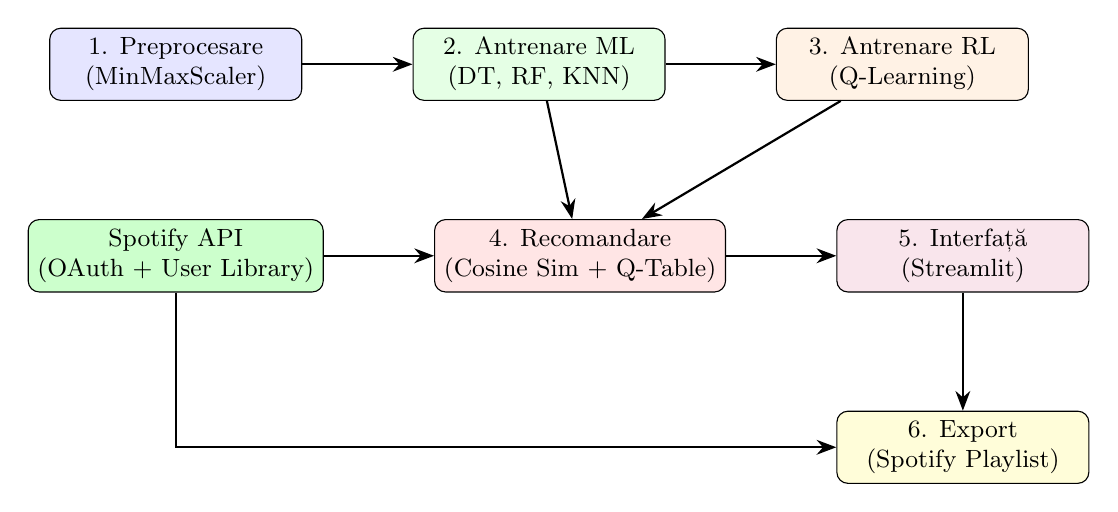
\begin{tikzpicture}[
    node distance=0.8cm and 1.4cm,
    box/.style={rectangle, draw, rounded corners, minimum width=3.2cm, minimum height=0.85cm, align=center, font=\small},
    arrow/.style={-{Stealth[length=2.5mm]}, thick}
]
    % Row 1: Training pipeline
    \node[box, fill=blue!10] (data) {1. Preprocesare\\(MinMaxScaler)};
    \node[box, fill=green!10, right=of data] (ml) {2. Antrenare ML\\(DT, RF, KNN)};
    \node[box, fill=orange!10, right=of ml] (rl) {3. Antrenare RL\\(Q-Learning)};

    % Row 2: Runtime pipeline
    \node[box, fill=green!20, below=1.5cm of data] (spotify) {Spotify API\\(OAuth + User Library)};
    \node[box, fill=red!10, right=of spotify] (rec) {4. Recomandare\\(Cosine Sim + Q-Table)};
    \node[box, fill=purple!10, right=of rec] (ui) {5. Interfață\\(Streamlit)};

    % Row 3: Output
    \node[box, fill=yellow!15, below=1.5cm of ui] (export) {6. Export\\(Spotify Playlist)};

    % Training arrows (row 1)
    \draw[arrow] (data) -- (ml);
    \draw[arrow] (ml) -- (rl);

    % Training -> Runtime (downward)
    \draw[arrow] (ml) -- (rec);
    \draw[arrow] (rl) -- (rec);
    \draw[arrow] (spotify) -- (rec);

    % Runtime flow
    \draw[arrow] (rec) -- (ui);

    % Output
    \draw[arrow] (ui) -- (export);
    \draw[arrow] (spotify) |- (export);
\end{tikzpicture}%
}
\caption{Arhitectura pipeline-ului Musicon cu integrare Spotify}
\label{fig:arhitectura}
\end{figure}

\subsection{Structura proiectului}

\begin{lstlisting}[language={}, caption={Structura fisierelor proiectului}]
Musicon/
  config.py              # Configuratie centrala
  preprocess.py          # Preprocesare date
  train.py               # Antrenare modele ML
  q_learning.py          # Antrenare agent RL
  recommender.py         # Generare playlist-uri
  streamlit_app.py       # Interfata web
  notebooks/             # Jupyter notebooks (EDA, ML, RL)
  data/
    raw/                 # Dataset original
    processed/           # Train/test split + scaler
  models/                # Modele antrenate (.pkl, .npy)
  results/               # Plot-uri si vizualizari
\end{lstlisting}

\subsection{Configurația centrală}

Toate constantele proiectului sunt definite în \texttt{config.py}: căile către fișiere, lista de feature-uri audio, cele 8 mood-uri cu codurile lor numerice, 24 de preset-uri de mood cu profiluri audio, setările ML și parametrii RL.

\FloatBarrier

% ═══════════════════════════════════════════════════════════════════
\section{Componenta de Machine Learning}
% ═══════════════════════════════════════════════════════════════════

\subsection{Dataset și preprocesare}
\label{sec:dataset}

\subsubsection{Sursa datelor}

Datasetul utilizat este \texttt{popular\_10k\_mood\_labeled.csv}, conținând \textbf{10.000 de piese} agregate din multiple surse Spotify. Fiecare piesă are 19 coloane, dintre care 8 reprezintă feature-uri audio relevante:

\begin{table}[H]
\centering
\caption{Feature-uri audio Spotify utilizate}
\label{tab:features}
\begin{tabular}{llc}
\toprule
\textbf{Feature} & \textbf{Descriere} & \textbf{Domeniu} \\
\midrule
danceability      & Potrivirea pentru dans              & $[0, 1]$ \\
energy            & Intensitate perceptuală             & $[0, 1]$ \\
loudness          & Volum general (dB)                  & $[-38.5, 1.0]$ \\
speechiness       & Prezența cuvintelor vorbite         & $[0, 1]$ \\
acousticness      & Încredere că piesa e acustică       & $[0, 1]$ \\
instrumentalness  & Absență vocală                      & $[0, 1]$ \\
valence           & Pozitivitate muzicală               & $[0, 1]$ \\
tempo             & Bătăi pe minut (BPM)                & $[0, 209]$ \\
\bottomrule
\end{tabular}
\end{table}

\subsubsection{Distribuția mood-urilor}

Datasetul folosește \textbf{8 categorii de mood} ordonate de-a lungul spectrului valență--energie:

\begin{table}[H]
\centering
\caption{Distribuția claselor de mood în dataset}
\label{tab:mood_dist}
\begin{tabular}{clr}
\toprule
\textbf{Cod} & \textbf{Mood} & \textbf{Număr piese} \\
\midrule
0 & melancholic & 867 \\
1 & dark        & 520 \\
2 & calm        & 246 \\
3 & nostalgic   & 790 \\
4 & romantic    & 117 \\
5 & happy       & 2\,951 \\
6 & euphoric    & 1\,919 \\
7 & energetic   & 2\,590 \\
\midrule
  & \textbf{Total} & \textbf{10\,000} \\
\bottomrule
\end{tabular}
\end{table}

Se observă un \textbf{dezechilibru de clasă} semnificativ: \textit{happy} și \textit{energetic} domină datasetul (55\% împreună), în timp ce \textit{romantic} (117) și \textit{calm} (246) sunt subreprezentate.

\subsubsection{Normalizare}

Feature-urile \texttt{loudness} (dB) și \texttt{tempo} (BPM) necesită normalizare la intervalul $[0, 1]$. Se utilizează \textbf{MinMaxScaler}:

\begin{equation}
x' = \frac{x - x_{\min}}{x_{\max} - x_{\min}}
\end{equation}

Celelalte 6 feature-uri sunt deja în $[0, 1]$, dar sunt trecute prin scaler pentru consistență.

\subsubsection{Împărțirea train/test}

Datasetul se împarte în \textbf{80\% train / 20\% test} cu stratificare pe coloana \texttt{mood\_code}, asigurând reprezentarea proporțională a tuturor celor 8 mood-uri în ambele subseturi. Scaler-ul antrenat este salvat pentru utilizare în faza de recomandare.

\FloatBarrier

\subsection{Clasificare}
\label{sec:clasificare}

\subsubsection{Modele antrenate}

S-au antrenat și comparat 3 clasificatori \cite{sklearn}:

\begin{enumerate}
    \item \textbf{Decision Tree} -- Adâncime maximă 8, ponderare automată a claselor (\text{class\_weight="balanced"})
    \item \textbf{Random Forest} \cite{breiman2001} -- 200 estimatori, adâncime maximă 12, ponderare automată
    \item \textbf{K-Nearest Neighbors (KNN)} \cite{fix1951} -- $k = 7$ vecini
\end{enumerate}

\subsubsection{Rezultate}

\begin{table}[H]
\centering
\caption{Comparația modelelor de clasificare}
\label{tab:results}
\begin{tabular}{lccc}
\toprule
\textbf{Model} & \textbf{Acuratețe test} & \textbf{CV medie (5-fold)} & \textbf{CV std} \\
\midrule
Decision Tree   & \textbf{0.9940} & 0.9917 & $\pm$0.0021 \\
Random Forest   & 0.9935          & 0.9915 & $\pm$0.0011 \\
KNN             & 0.8605          & 0.8557 & $\pm$0.0089 \\
\bottomrule
\end{tabular}
\end{table}

Pentru a valida robustetea rezultatelor, s-a aplicat \textbf{5-fold cross-validation stratificat}. Deviația standard mică ($\leq 0.009$) confirmă că acuratețea este stabilă pe toate fold-urile, nu doar pe un split particular.

\subsubsection{Metrici per clasă}

Pentru a evalua impactul dezechilibrului de clasă, tabelul următor prezintă metricile detaliate pentru cel mai bun model (Decision Tree):

\begin{table}[H]
\centering
\caption{Metrici per clasă -- Decision Tree (test)}
\label{tab:perclass}
\small
\begin{tabular}{lrrrr}
\toprule
\textbf{Mood} & \textbf{Suport} & \textbf{Precizie} & \textbf{Recall} & \textbf{F1} \\
\midrule
melancholic (0) & 173 & 0.99 & 1.00 & 1.00 \\
dark (1)        & 104 & 0.99 & 0.99 & 0.99 \\
calm (2)        &  49 & 0.94 & 0.94 & 0.94 \\
nostalgic (3)   & 158 & 0.99 & 0.97 & 0.98 \\
romantic (4)    &  24 & 0.92 & 1.00 & 0.96 \\
happy (5)       & 590 & 1.00 & 1.00 & 1.00 \\
euphoric (6)    & 384 & 1.00 & 1.00 & 1.00 \\
energetic (7)   & 518 & 1.00 & 1.00 & 1.00 \\
\bottomrule
\end{tabular}
\end{table}

Se observă că, deși clasele minoritare (\textit{romantic}=24, \textit{calm}=49) au suport redus, parametrul \texttt{class\_weight="balanced"} menține precizia peste 92\% și recall la 94--100\%.

\begin{figure}[H]
\centering
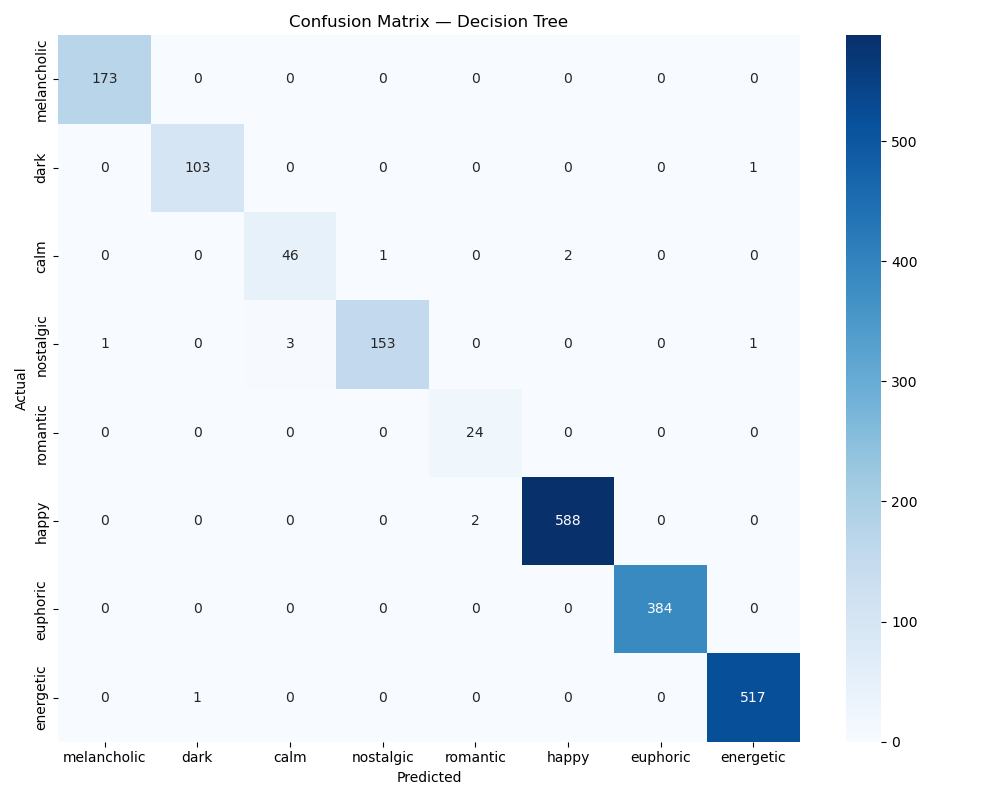
\includegraphics[width=0.8\textwidth]{results/confusion_matrix_decision_tree.png}
\caption{Matricea de confuzie pentru cel mai bun model (Decision Tree)}
\label{fig:confusion}
\end{figure}

\begin{figure}[H]
\centering
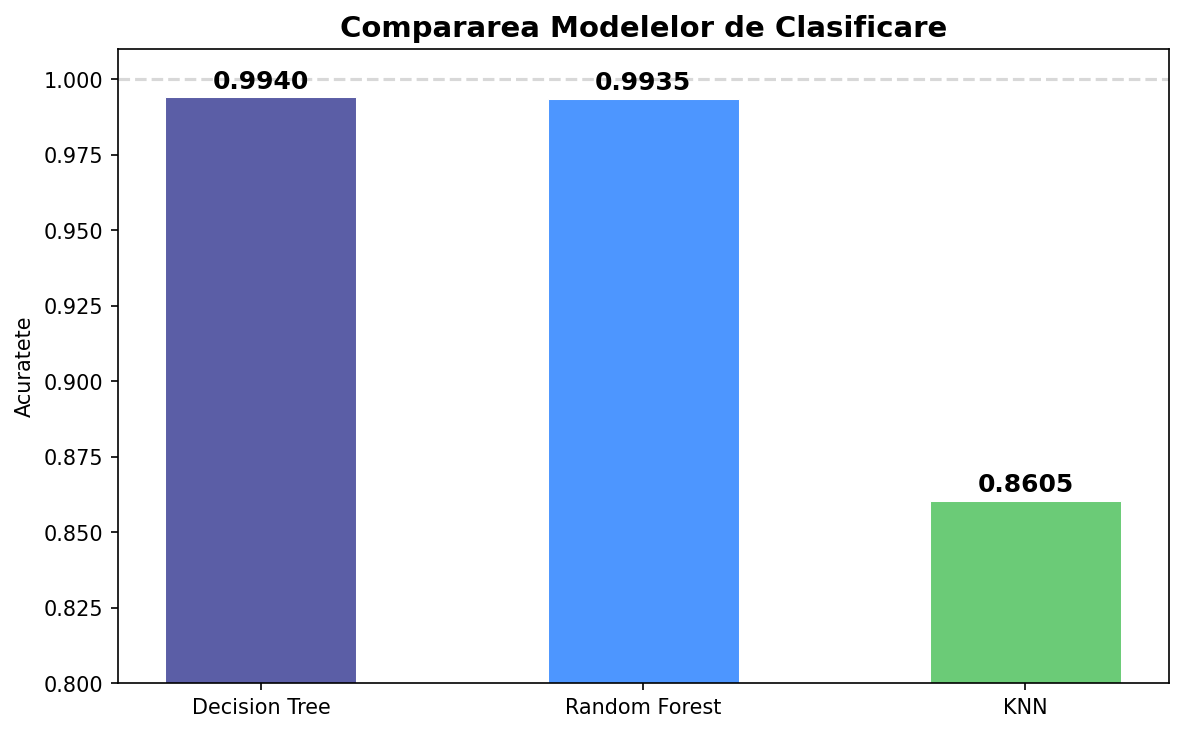
\includegraphics[width=0.7\textwidth]{results/model_comparison.png}
\caption{Comparația acurateții celor 3 modele de clasificare}
\label{fig:model_comparison}
\end{figure}

\begin{figure}[H]
\centering
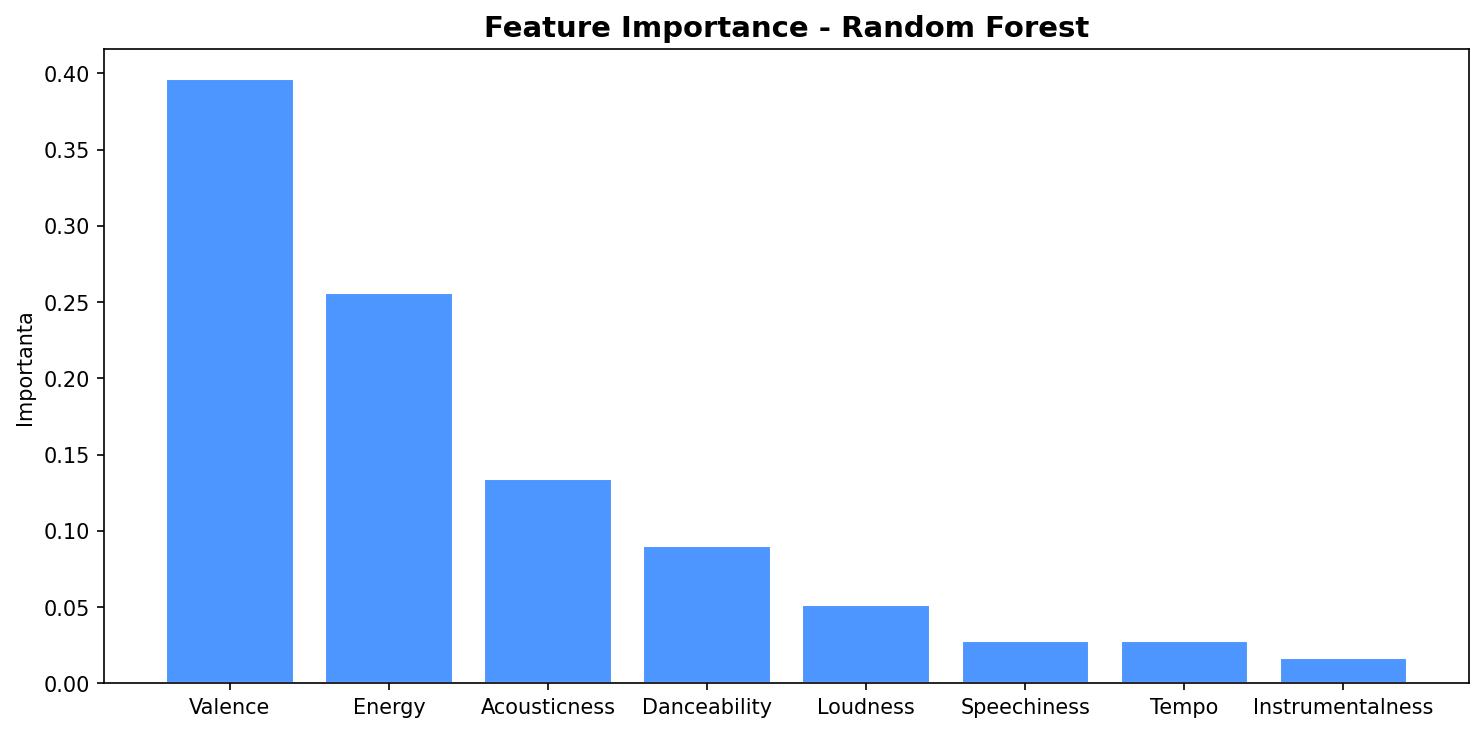
\includegraphics[width=0.8\textwidth]{results/feature_importance.png}
\caption{Importanța feature-urilor audio în modelul Random Forest}
\label{fig:feature_importance}
\end{figure}

\subsubsection{Analiza acurateții ridicate}

Acuratețea de 99.40\% provine din modul în care au fost generate labelurile pentru mood. Acestea au fost asignate \textbf{deterministic pe baza feature-urilor audio} (reguli pe valență, energie etc.). Clasificatorul învață în mod eficient aceleași reguli din date.

Acest fenomen este valabil și pentru Random Forest (0.9935), care este un ansamblu de arbori de decizie. KNN obține un scor mai scăzut (0.8605) deoarece este un clasificator bazat pe instanțe și poate greși în alegerea dintre mood-urile adiacente.

Validarea prin \textbf{5-fold cross-validation stratificat} confirmă că rezultatele sunt consistente (CV std $\leq 0.009$), eliminând posibilitatea unui overfitting pe un anumit split. De asemenea, parametrul \texttt{max\_depth=8} limitează complexitatea arborilor, iar \texttt{class\_weight="balanced"} compensează dezechilibrul de clasă, menținând metricile per clasă peste 92\% inclusiv pentru categoriile minoritare.

\FloatBarrier

\subsection{Comparația supervizat vs.\ nesupervizat}

În versiunile anterioare ale proiectului s-a comparat și abordarea nesupervizată (K-Means Clustering). Clusterele K-Means nu aliniau perfect cele 8 mood-uri, confirmând că etichetarea deterministă pe feature-uri oferă o separare superioară față de gruparea nesupervizată.

\FloatBarrier

% ═══════════════════════════════════════════════════════════════════
\section{Componenta de Reinforcement Learning}
% ═══════════════════════════════════════════════════════════════════

\subsection{Formularea MDP}
\label{sec:mdp}

Problema generării unui playlist este formulată ca un \textbf{Proces Decizional Markov (MDP)} definit prin tuplul $(S, A, T, R, \gamma)$.

\subsubsection{Spațiul stărilor}

O stare este definită ca un triplet:

\begin{equation}
s = (\text{mood\_curent}, \text{mood\_tinta}, \text{bucket\_pozitie})
\end{equation}

\begin{itemize}
    \item \textbf{mood\_curent} $\in \{0, 1, ..., 7\}$ -- mood-ul ultimei piese selectate;
    \item \textbf{mood\_țintă} $\in \{0, 1, ..., 7\}$ -- mood-ul dorit de utilizator;
    \item \textbf{bucket\_poziție} $\in \{0, 1, 2\}$ -- segmentul playlist-ului:
    \begin{itemize}
        \item 0: început (pozițiile 0--3);
        \item 1: mijloc (pozițiile 4--7);
        \item 2: final (pozițiile 8--9).
    \end{itemize}
\end{itemize}

\textbf{Spațiu total de stări:} $|S| = 8 \times 8 \times 3 = 192$

\subsubsection{Spațiul acțiunilor}

O acțiune $a \in \{0, 1, ..., 9\}$ reprezintă selecția unuia dintre cei 10 candidați din pool-ul de piese.

\subsubsection{Funcția de recompensă}

\begin{equation}
R(s, a) = \begin{cases}
1.0 & \text{dacă mood-ul piesei selectate = mood\_țintă} \\
0.5 & \text{dacă mood-ul piesei este adiacent mood-ului țintă} \\
0.0 & \text{altfel}
\end{cases}
\end{equation}

\textbf{Adiacența} între mood-uri este definită pe spectrul valență--energie:

\begin{table}[H]
\centering
\caption{Mood-uri adiacente}
\label{tab:adjacent}
\begin{tabular}{cl}
\toprule
\textbf{Mood} & \textbf{Adiacente} \\
\midrule
0 (melancholic) & nostalgic, calm \\
1 (dark)        & energetic, melancholic \\
2 (calm)        & nostalgic, melancholic \\
3 (nostalgic)   & melancholic, romantic \\
4 (romantic)    & nostalgic, happy \\
5 (happy)       & romantic, euphoric \\
6 (euphoric)    & happy, energetic \\
7 (energetic)   & euphoric, dark \\
\bottomrule
\end{tabular}
\end{table}

\FloatBarrier

\subsection{Antrenarea Q-Learning}
\label{sec:qlearning}

Algoritmul Q-Learning \cite{watkins1992}, formulat în cadrul teoriei învățării prin recompensă \cite{sutton2018}, actualizează o tabelă Q de dimensiune $192 \times 10$ folosind regula:

\begin{equation}
Q(s, a) \leftarrow Q(s, a) + \alpha \left[ R(s, a) + \gamma \max_{a'} Q(s', a') - Q(s, a) \right]
\label{eq:qupdate}
\end{equation}

\textbf{Hiperparametri:}

\begin{table}[H]
\centering
\caption{Hiperparametrii Q-Learning}
\label{tab:rl_params}
\begin{tabular}{llc}
\toprule
\textbf{Parametru} & \textbf{Simbol} & \textbf{Valoare} \\
\midrule
Rata de învățare      & $\alpha$          & 0.1 \\
Factorul de discount  & $\gamma$          & 0.95 \\
Epsilon inițial       & $\epsilon_0$      & 1.0 \\
Decay epsilon         & $\epsilon_d$      & 0.995 \\
Epsilon minim         & $\epsilon_{\min}$ & 0.01 \\
Număr episoade        & --                & 2\,000 \\
Lungime playlist      & --                & 10 \\
\bottomrule
\end{tabular}
\end{table}

Strategia $\epsilon$-greedy asigură explorare în primele episoade ($\epsilon = 1.0$) și trecerea graduală spre exploatare pe măsură ce $\epsilon$ scade la $\epsilon_{\min} = 0.01$.

\FloatBarrier

\subsection{Analiza convergenței}

\begin{figure}[H]
\centering
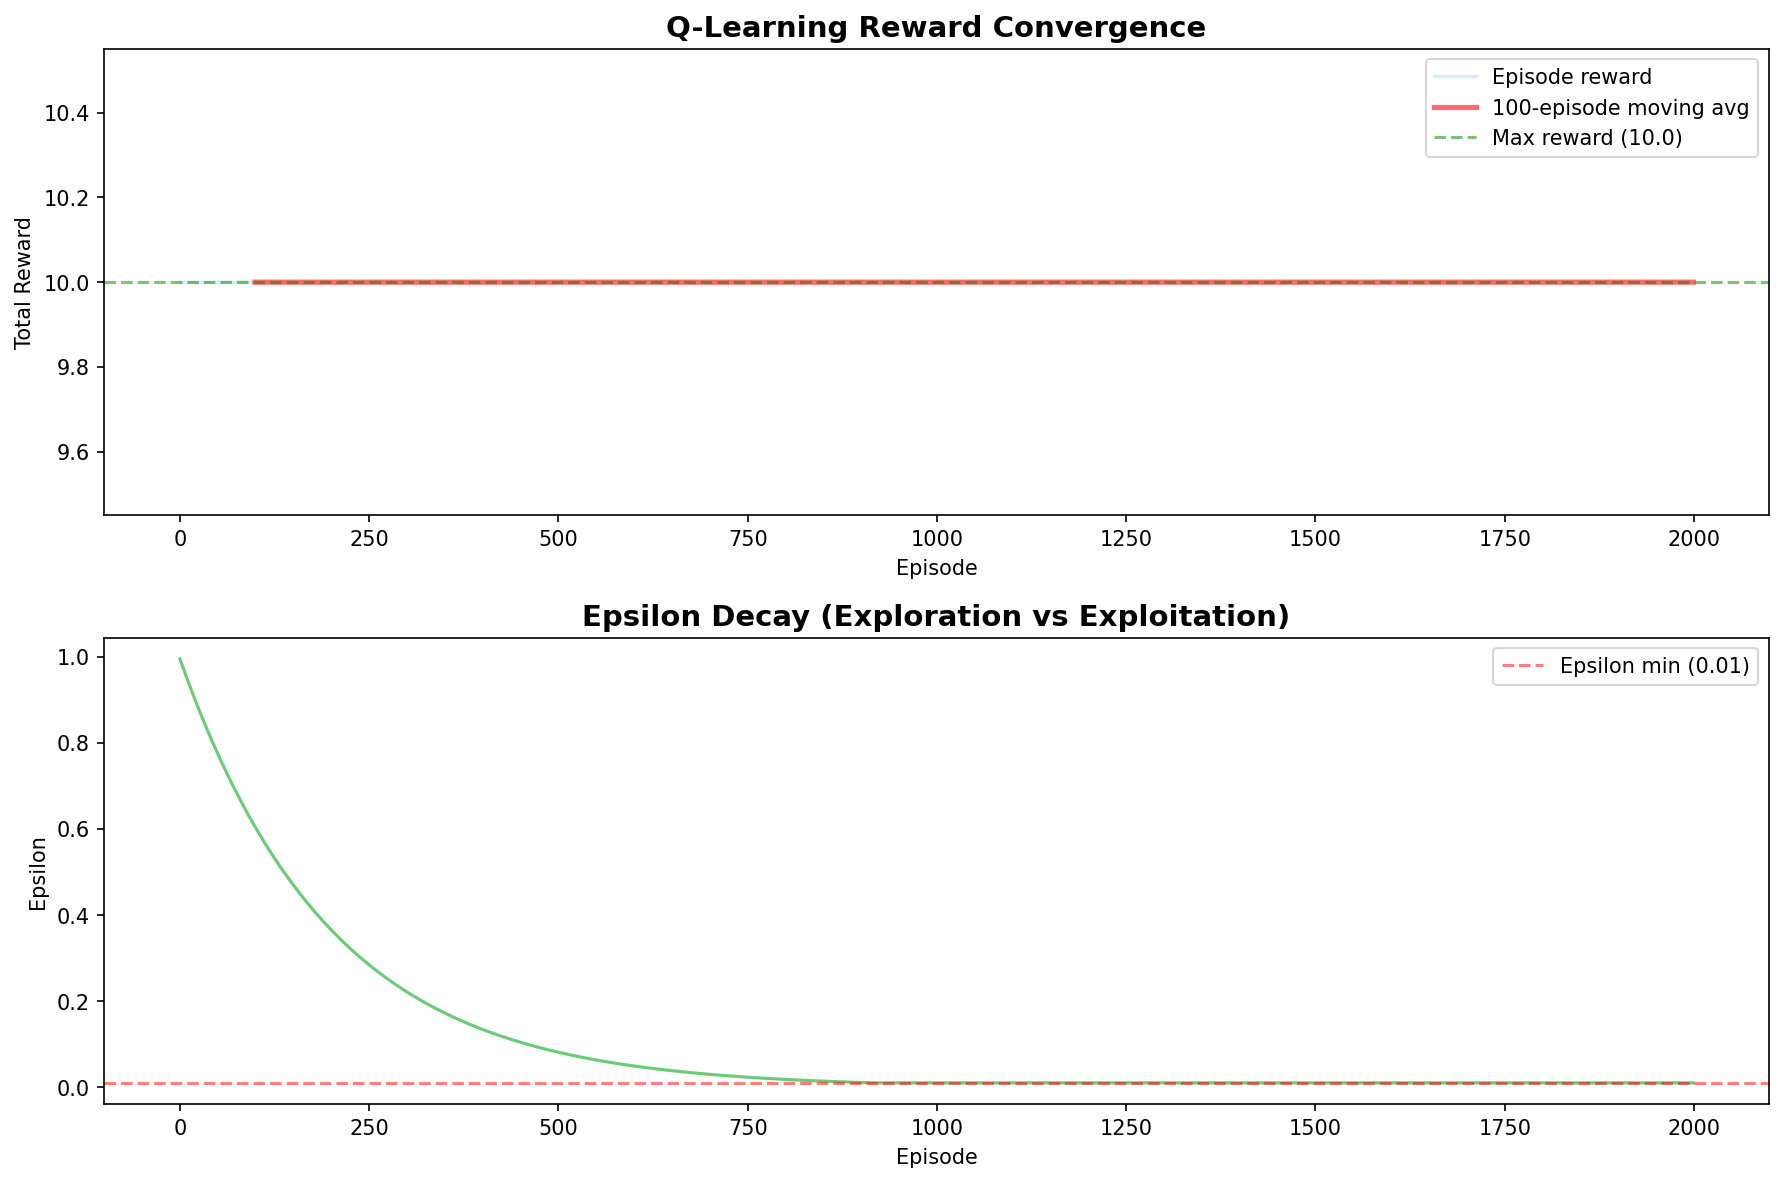
\includegraphics[width=0.9\textwidth]{results/reward_curve.png}
\caption{Curba de convergență a recompensei Q-Learning}
\label{fig:reward_curve}
\end{figure}

Rezultatele antrenării:
\begin{itemize}
    \item \textbf{Episoade completate:} 2\,000
    \item \textbf{Epsilon final:} 0.0100
    \item \textbf{Recompensă medie (ultimele 100 episoade):} 10.00
\end{itemize}

Recompensa maximă teoretică pe episod este $10.0$ (10 poziții $\times$ recompensă 1.0). Agentul atinge această limită, confirmând \textbf{convergența completă} a politicii învățate. Acest rezultat este consistent cu acuratețea ridicată a clasificatorului ML: deoarece piesele sunt corect etichetate în proporție de 99.4\%, agentul RL poate găsi întotdeauna o secvență optimă.

\begin{figure}[H]
\centering
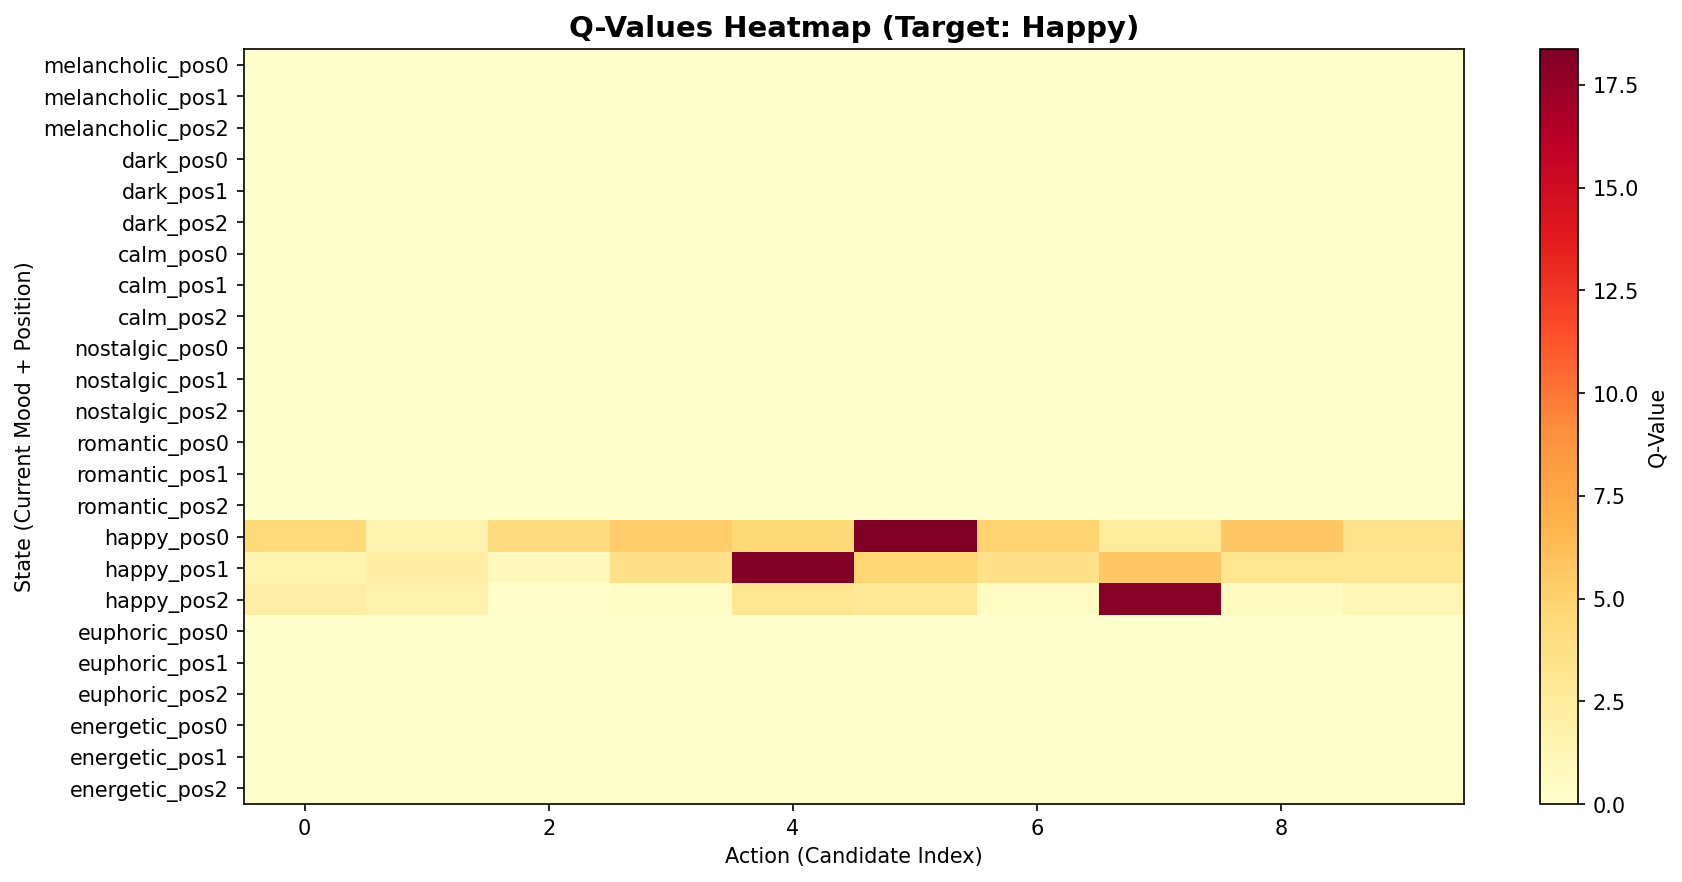
\includegraphics[width=0.85\textwidth]{results/q_table_heatmap.png}
\caption{Hartă termică a Q-Table-ului pentru mood-ul țintă happy (stări $\times$ acțiuni)}
\label{fig:q_heatmap}
\end{figure}

\FloatBarrier

\subsection{Învățare online prin feedback-ul utilizatorului}
\label{sec:feedback}

Politica pre-antrenată produce playlist-uri optime din punct de vedere al mood-ului, dar nu ține cont de preferințele individuale ale utilizatorului. Pentru a face componenta RL cu adevărat adaptivă, am implementat un mecanism de \textbf{feedback online} care permite utilizatorului să evalueze fiecare piesă din playlist cu \textbf{Like} sau \textbf{Dislike}. Acest feedback actualizează Q-Table-ul în timp real, astfel încât generările ulterioare produc playlist-uri adaptate la gustul utilizatorului.

\subsubsection{Mecanismul de actualizare}

Pentru fiecare piesă evaluată, sistemul identifică starea $s = (mood\_curent, mood\_tinta, pozitie)$ și acțiunea $a$ care a fost selectată, apoi actualizează valoarea Q corespunzătoare:

\begin{equation}
Q(s, a) \leftarrow
\begin{cases}
Q(s, a) + \alpha \cdot (1.0 - Q(s, a)) & \text{dacă Like} \\
Q(s, a) - \alpha \cdot Q(s, a) & \text{dacă Dislike}
\end{cases}
\label{eq:feedback}
\end{equation}

unde $\alpha = 0.1$ este rata de învățare. Această formulă asigură că:
\begin{itemize}
    \item \textbf{Like-ul} crește gradual valoarea $Q(s, a)$ spre $1.0$, întărind selecția acelei acțiuni în starea respectivă;
    \item \textbf{Dislike-ul} scade valoarea $Q(s, a)$ spre $0.0$, penalizând acțiunea și făcând ca alte piese să fie preferate la următoarea generare.
\end{itemize}

Q-Table-ul este salvat pe disc după fiecare rundă de feedback, deci preferințele se acumulează între sesiuni.

\subsubsection{Fluxul interactiv}

\begin{enumerate}
    \item Utilizatorul generează un playlist inițial (bazat pe politica pre-antrenată);
    \item Evaluează fiecare piesă cu \textbf{Like} sau \textbf{Dislike} din interfața Streamlit;
    \item Apasă ``Send Feedback'' -- Q-Table-ul se actualizează și se salvează;
    \item Generează din nou același preset -- playlist-ul reflectă acum preferințele utilizatorului.
\end{enumerate}

Acest mecanism transformă agentul RL dintr-un selector static într-un \textbf{sistem adaptiv} care învață continuu din interacțiunea cu utilizatorul. Fiecare rundă de feedback modifică politicile de selecție, rezultând playlist-uri progresiv mai aliniate cu gusturile individuale.

\begin{figure}[H]
\centering
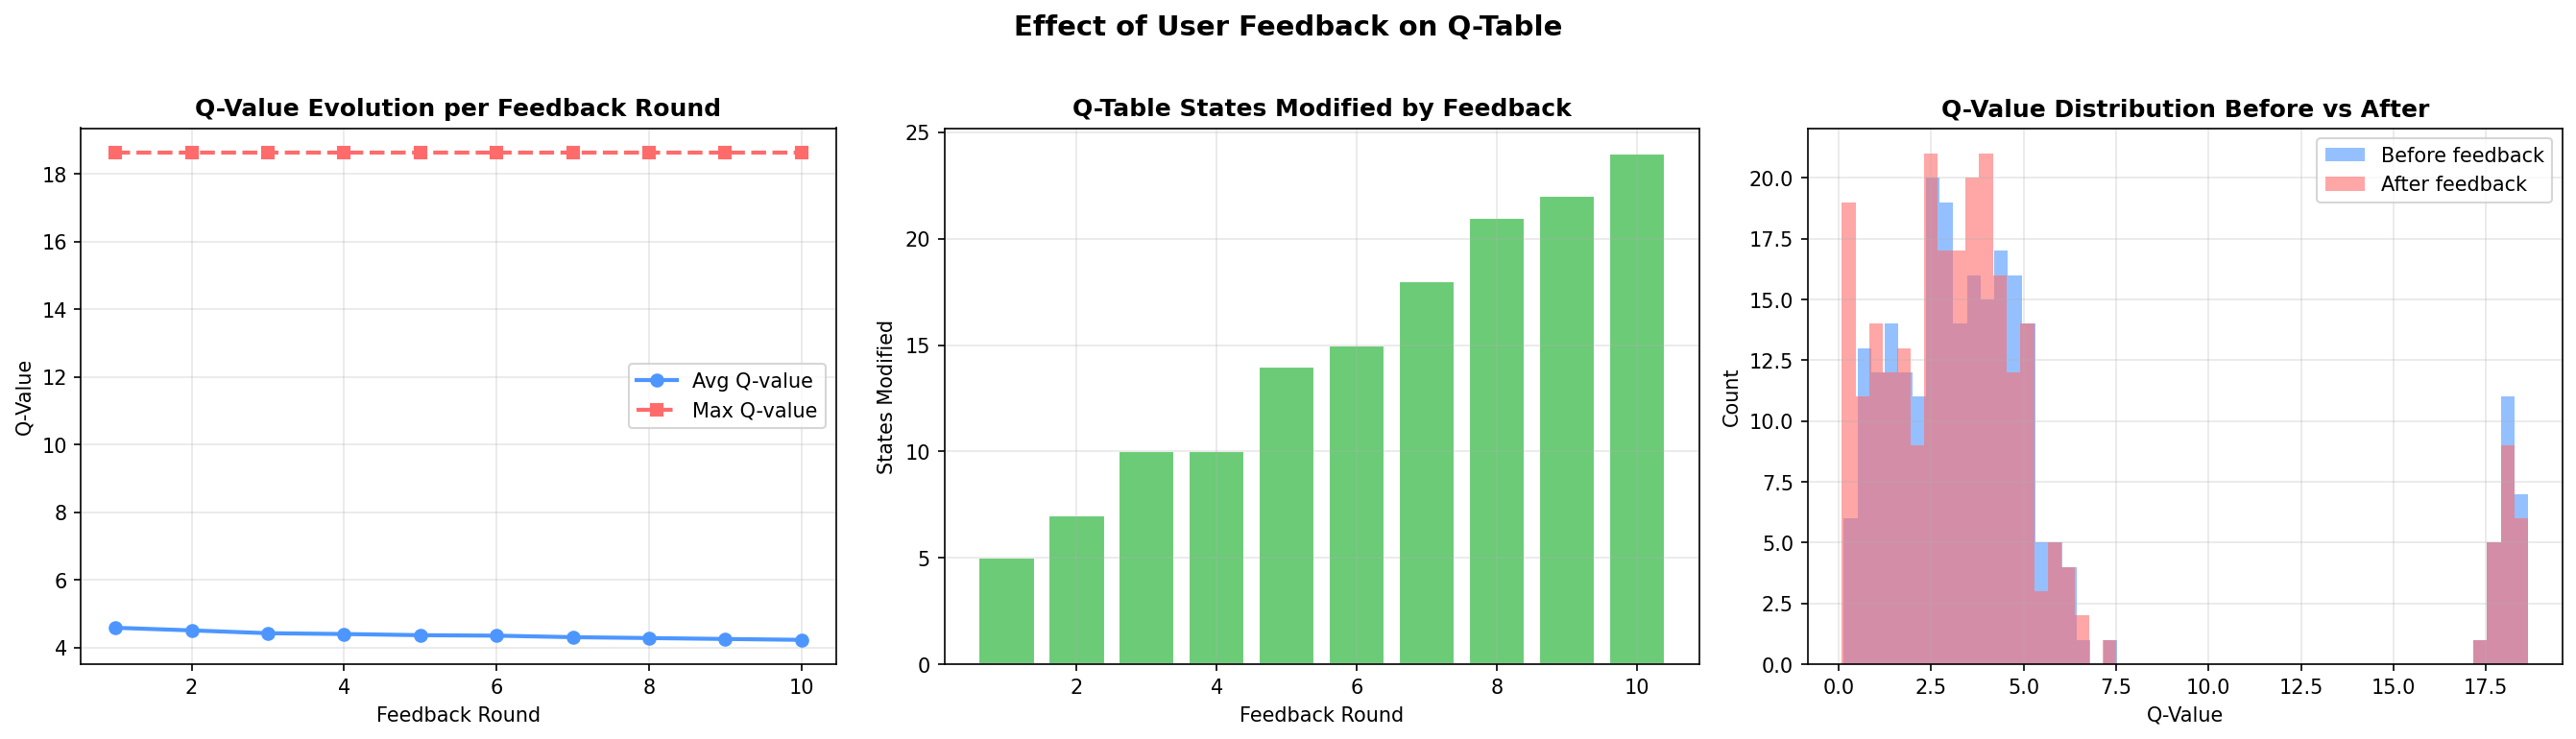
\includegraphics[width=0.9\textwidth]{results/feedback_effect.png}
\caption{Efectul feedback-ului utilizatorului asupra Q-Table-ului: evoluția Q-values, stări modificate și distribuția înainte/după}
\label{fig:feedback_effect}
\end{figure}

\FloatBarrier

% ═══════════════════════════════════════════════════════════════════
\section{Integrarea componentelor}
% ═══════════════════════════════════════════════════════════════════

Modulul \texttt{recommender.py} integrează toate componentele într-un pipeline unitar:

\begin{enumerate}
    \item \textbf{Selecția preset-ului} -- Utilizatorul alege un preset de mood (sau descrie textual). Din cele 24 de preset-uri, fiecare are un profil audio definit.

    \item \textbf{Potrivirea prin similaritate cosinus} -- Profilul preset-ului este normalizat cu scaler-ul salvat, apoi se calculează similaritatea cosinus față de toate cele 10.000 de piese:

    \begin{equation}
    \text{sim}(\mathbf{p}, \mathbf{s}) = \frac{\mathbf{p} \cdot \mathbf{s}}{\|\mathbf{p}\| \cdot \|\mathbf{s}\|}
    \end{equation}

    Se păstrează top 100 cele mai similare piese.

    \item \textbf{Clasificarea mood-ului} -- Modelul ML (Decision Tree, 99.4\% acuratețe) prezice mood-ul fiecărui candidat. Dacă sub 20 de candidați au mood-ul țintă, se suplimentează cu piese din întregul dataset.

    \item \textbf{Selecția prin Q-Table} -- Pentru fiecare din cele 10 poziții din playlist:
    \begin{enumerate}
        \item Se codifică starea curentă $(mood\_curent, mood\_tinta, bucket\_pozitie)$;
        \item Se construiește un pool de 10 candidați (jumătate cu mood țintă, restul diverși);
        \item Se selectează acțiunea $a^* = \arg\max_a Q(s, a)$;
        \item Piesa selectată devine noul \texttt{mood\_curent}.
    \end{enumerate}

    \item \textbf{Returnare} -- Playlist-ul final conține 10 piese cu track\_name, artist, genre, year, mood, similarity și cele 8 feature-uri audio.
\end{enumerate}

\FloatBarrier

% ═══════════════════════════════════════════════════════════════════
\section{Interfața cu utilizatorul}
% ═══════════════════════════════════════════════════════════════════

Interfața este construită cu \textbf{Streamlit} \cite{streamlit} și oferă o experiență vizuală modernă cu temă dark și animații CSS.

\subsection{Funcționalități}

\begin{itemize}
    \item \textbf{Selecție prin preset-uri} -- 24 de butoane grupate în 4 coloane, câte 2 mood-uri pe coloană
    \item \textbf{Text liber} -- Input text pentru descrierea mood-ului, mapat prin keyword matching;
    \item \textbf{Generare playlist} -- Apelul funcției \texttt{generate\_playlist()} cu spinner vizual;
    \item \textbf{Afișare playlist} -- Fiecare piesă afișată cu nume, artist, gen, an, procent de similaritate și badge colorat pentru mood;
    \item \textbf{Analiza feature-urilor} -- Grafic radar polar (Plotly) cu cele 8 feature-uri medii și valori individuale;
    \item \textbf{Secțiunea ``How it works''} -- Explicație vizuală a pipeline-ului în 4 pași;
    \item \textbf{Feedback RL} -- Evaluare Like/Dislike per piesă, cu actualizare Q-Table în timp real (detalii în Secțiunea~\ref{sec:feedback});
    \item \textbf{Integrare Spotify} -- Conectarea contului Spotify pentru personalizarea playlist-urilor (detalii în Secțiunea~\ref{sec:spotify});
    \item \textbf{Export pe Spotify} -- Crearea unui playlist public direct pe contul utilizatorului cu piesele generate.
\end{itemize}

\subsection{Lansarea aplicației}

\begin{lstlisting}[language=bash, caption={Comanda de lansare}]
python3 -m streamlit run streamlit_app.py
\end{lstlisting}

\FloatBarrier

% ═══════════════════════════════════════════════════════════════════
\section{Integrarea cu Spotify}
\label{sec:spotify}
% ═══════════════════════════════════════════════════════════════════

Pentru a personaliza recomandările, aplicația oferă opțional conectarea contului Spotify al utilizatorului prin \textbf{Spotify Web API} \cite{spotifyapi}. Această integrare permite sistemului să folosească istoricul de ascultare pentru a ajusta profilul audio al playlist-ului generat.

\subsection{Fluxul de autentificare OAuth 2.0}

Autentificarea utilizează protocolul \textbf{OAuth 2.0 Authorization Code Flow} prin biblioteca \texttt{spotipy}. Fluxul presupune următorii pași:

\begin{enumerate}
    \item Utilizatorul apasă butonul ``Connect Spotify'' în interfața Streamlit
    \item Aplicația generează un URL de autorizare Spotify cu scope-ul \texttt{user-library-read user-top-read}
    \item Utilizatorul este redirecționat către pagina de autentificare Spotify, unde aprobă accesul
    \item Spotify redirecționează către o pagină de callback găzduită pe GitHub Pages 
    \item Pagina de callback extrage codul de autorizare din URL și redirecționează către instanța locală Streamlit
    \item Aplicația face exchange pe cod pentru un access token și creează un client Spotify autentificat
\end{enumerate}

\begin{lstlisting}[caption={Crearea clientului Spotify autentificat}]
from spotipy.oauth2 import SpotifyOAuth

auth_manager = SpotifyOAuth(
    client_id=SPOTIPY_CLIENT_ID,
    client_secret=SPOTIPY_CLIENT_SECRET,
    redirect_uri=SPOTIPY_REDIRECT_URI,
    scope="user-library-read user-top-read playlist-modify-public",
)
token_info = auth_manager.get_access_token(code, as_dict=True)
sp = spotipy.Spotify(auth=token_info["access_token"])
\end{lstlisting}

\subsection{Extragerea bibliotecii utilizatorului}

După autentificare, funcția \texttt{get\_user\_songs\_from\_spotify()} extrage piese din două surse:

\begin{itemize}
    \item \textbf{Saved Tracks} -- Ultimele 50 de piese salvate în biblioteca Spotify;
    \item \textbf{Top Tracks} -- Top 50 piese pe termen mediu (\texttt{time\_range="medium\_term"}).
\end{itemize}

Piesele sunt deduplicate și apoi \textbf{potrivite cu datasetul local} prin compararea \texttt{track\_name} și \texttt{artist} (case-insensitive). Piesele utilizatorului care există în dataset rețin feature-urile audio normalizate.

\begin{lstlisting}[caption={Potrivirea pieselor Spotify cu datasetul local}]
for s in unique_user_songs:
    mask = (df["track_name"].str.lower() == s["track_name"].lower()) & \
           (df["artist"].str.lower() == s["artist"].lower())
    if mask.any():
        matched.append(df.loc[mask].iloc[0])
\end{lstlisting}

\subsection{Fuziunea profilurilor audio}

La generare se folosește un profil audio \textbf{hibrid} care îmbină preferințele utilizatorului cu preset-ul selectat:

\begin{equation}
\text{profile}_{\text{blended}} = 0.6 \times \text{profile}_{\text{preset}} + 0.4 \times \text{profile}_{\text{user}}
\end{equation}

unde $\text{profile}_{\text{user}}$ este media feature-urilor audio ale pieselor potrivite din biblioteca utilizatorului. Această fuziune asigură că playlist-ul păstrează caracterul mood-ului selectat, dar este influențat de gusturile personale.

Dacă utilizatorul nu conectează Spotify, sistemul folosește exclusiv profilul preset-ului.

\subsection{Detalii de implementare}

Starea conexiunii Spotify este gestionată prin \texttt{st.session\_state}, cu următoarele chei:

\begin{table}[H]
\centering
\caption{Session state pentru integrarea Spotify}
\label{tab:spotify_state}
\begin{tabular}{ll}
\toprule
\textbf{Cheie} & \textbf{Descriere} \\
\midrule
\texttt{sp\_user}            & Client spotipy autentificat \\
\texttt{user\_songs}         & DataFrame cu piesele potrivite \\
\texttt{spotify\_connected}  & Flag boolean pentru stare conexiune \\
\texttt{spotify\_song\_count} & Numărul de piese potrivite \\
\bottomrule
\end{tabular}
\end{table}

Parametrii de conectare (client ID, client secret, redirect URI) sunt stocați în \texttt{config.py} și încărcați la inițializarea aplicației.

\subsection{Exportul playlist-ului pe Spotify}

După generarea playlist-ului, utilizatorul poate exporta direct lista de piese pe contul său Spotify. Funcția \texttt{export\_playlist\_to\_spotify()} realizează următorii pași:

\begin{enumerate}
    \item Creează un nou playlist public pe contul utilizatorului prin \texttt{user\_playlist\_create()};
    \item Pentru fiecare piesă din playlist-ul generat, caută pe Spotify după nume și artist folosind \texttt{sp.search()};
    \item Dacă prima căutare nu returnează rezultate, reîncearcă cu un query mai larg (doar numele piesei);
    \item Adaugă toate piesele găsite (ca URI-uri Spotify) în playlist-ul nou creat prin \texttt{user\_playlist\_add\_tracks()};
    \item Returnează URL-ul playlist-ului, numărul de piese găsite și lista pieselor negăsite.
\end{enumerate}

Scope-ul OAuth necesar include \texttt{playlist-modify-public} pentru crearea și popularea playlist-ului. Interfața afișează un buton ``Export to Spotify'' doar dacă utilizatorul este conectat și a generat deja un playlist.

\FloatBarrier

% ═══════════════════════════════════════════════════════════════════
\section{Concluzii și direcții viitoare}
% ═══════════════════════════════════════════════════════════════════

\subsection{Concluzii}

Proiectul Musicon demonstrează cu succes integrarea a două paradigme de Inteligență Artificială pentru generarea de playlist-uri bazate pe mood:

\begin{enumerate}
    \item \textbf{Clasificarea ML} obține acuratețe excepțională (99.4\%) validată prin 5-fold cross-validation stratificat (CV std $\pm$0.0021), confirmând robustetea modelelor. Parametrul \texttt{class\_weight="balanced"} asigură metrici per clasă peste 92\% inclusiv pentru categoriile minoritare.

    \item \textbf{Agentul Q-Learning} converge la politica optimă (recompensă 10.0/10.0) în 2.000 de episoade, validând formularea MDP cu 192 de stări și sistemul de recompensă cu adiacență.

    \item \textbf{Integrarea} între similaritatea cosinus, clasificarea ML și selecția RL produce playlist-uri coerente, cu piese relevante pentru mood-ul selectat.

    \item \textbf{Feedback-ul online} permite utilizatorului să evalueze fiecare piesă (Like/Dislike), actualizând Q-Table-ul în timp real și transformând agentul RL într-un sistem adaptiv care învață din preferințele individuale.

    \item \textbf{Integrarea Spotify} permite personalizarea recomandărilor prin fuziunea profilului audio al utilizatorului cu cel al preset-ului selectat, plus exportul direct al playlist-ului pe contul Spotify.

    \item \textbf{Interfața Streamlit} oferă o experiență utilizator modernă și intuitivă, cu autentificare OAuth 2.0 pentru conectarea la Spotify și export direct de playlist-uri.
\end{enumerate}

\subsection{Direcții viitoare}

\begin{itemize}
    \item \textbf{Deep Learning} -- Înlocuirea clasificatorului cu o rețea neuronală pentru o mai bună generalizare pe dataset-uri cu etichete nedeterministe;
    \item \textbf{NLP pentru detecția mood-ului} -- Utilizarea unui model de procesare a limbajului natural pentru interpretarea textului liber, în loc de keyword matching;
    \item \textbf{Extinderea taxonomiei} -- Trecerea de la 8 la 16+ mood-uri pentru o și mai mare nuanță emoțională;
    \item \textbf{Deployment} -- Publicarea aplicației pe Streamlit Cloud pentru acces public.
\end{itemize}


% ═══════════════════════════════════════════════════════════════════
\section{Bibliografie}
% ═══════════════════════════════════════════════════════════════════

\begin{thebibliography}{9}

\bibitem{russell1980}
J.\ A.\ Russell, ``A circumplex model of affect,'' \textit{Journal of Personality and Social Psychology}, vol.~39, nr.~6, pp.~1161--1178, 1980.

\bibitem{thayer1989}
R.\ E.\ Thayer, \textit{The Biopsychology of Mood and Arousal}. Oxford University Press, 1989.

\bibitem{watkins1992}
C.\ J.\ C.\ H.\ Watkins, ``Q-learning,'' \textit{Machine Learning}, vol.~8, nr.~3, pp.~279--292, 1992.

\bibitem{sutton2018}
R.\ S.\ Sutton și A.\ G.\ Barto, \textit{Reinforcement Learning: An Introduction}, 2nd~ed. MIT Press, 2018.

\bibitem{sklearn}
F.\ Pedregosa et~al., ``Scikit-learn: Machine learning in Python,'' \textit{Journal of Machine Learning Research}, vol.~12, pp.~2825--2830, 2011.

\bibitem{streamlit}
Streamlit Inc., ``Streamlit: The fastest way to build and share data apps,'' \url{https://streamlit.io}, 2024.

\bibitem{spotifyapi}
Spotify, ``Spotify Web API Reference,'' \url{https://developer.spotify.com/documentation/web-api}, 2024.

\bibitem{breiman2001}
L.\ Breiman, ``Random forests,'' \textit{Machine Learning}, vol.~45, nr.~1, pp.~5--32, 2001.

\bibitem{fix1951}
E.\ Fix și J.\ L.\ Hodges, ``Discriminatory analysis: Nonparametric discrimination: Consistency properties,'' USAF School of Aviation Medicine, Technical Report 4, 1951.

\bibitem{aggarwal2016}
C.\ C.\ Aggarwal, \textit{Recommender Systems: The Textbook}. Springer, 2016.

\bibitem{moodify2026}
S.\ Weiss, ``Moodify -- ML Hybrid Music Recommender System,'' \url{https://github.com/Sabriweiss/MOODIFY}, 2026.

\bibitem{moodify2023}
Orzanai, ``Moodify -- Emotion Recognition \& Recommendation using LGBM and Cosine Similarity,'' \url{https://github.com/orzanai/Moodify}, 2023.

\bibitem{moodify2024devpost}
Moodify Team, ``Moodify -- AI-Powered Mood-Based Playlist Generator,'' \url{https://devpost.com/software/moodify-ai-powered-mood-based-playlist-generator}, 2024.

\bibitem{moodify2024chrome}
Moodify AI, ``Moodify AI -- Playlist generator in Spotify (Chrome Extension),'' \url{https://chromewebstore.google.com/detail/moodify-ai-playlist-gener/ojndmbgkbjbffkphfinoncblkimodgme}, 2024.

\end{thebibliography}


% ═══════════════════════════════════════════════════════════════════
\section{Manual de utilizare}
% ═══════════════════════════════════════════════════════════════════

\subsection{Cerințe de sistem}

\begin{itemize}
    \item Python 3.10+
    \item Bibliotecile din \texttt{requirements.txt}
\end{itemize}

\subsection{Instalare}

\begin{lstlisting}[language=bash, caption={Instalarea dependintelor}]
pip install -r requirements.txt
\end{lstlisting}

\subsection{Pipeline-ul de antrenare}

\begin{lstlisting}[language=bash, caption={Rularea pipeline-ului}]
# Pasul 1: Preprocesare date
python3 preprocess.py

# Pasul 2: Antrenare modele ML
python3 train.py

# Pasul 3: Antrenare Q-Learning
python3 q_learning.py
\end{lstlisting}

\subsection{Lansarea interfeței}

\begin{lstlisting}[language=bash, caption={Lansarea aplicatiei}]
python3 -m streamlit run streamlit_app.py
\end{lstlisting}

Aplicația se deschide în browser la \texttt{http://localhost:8502}.

\subsection{Utilizare}

\begin{enumerate}
    \item Selectați un mood din cele 24 de preset-uri afișate, SAU tastați o descriere în câmpul de text;
    \item (Opțional) Expandați secțiunea ``Spotify Integration'' și apăsați ``Connect Spotify'' pentru a vă conecta contul. Aplicația va extrage automat piesele din biblioteca dvs.;
    \item Apăsați butonul ``Generate Playlist'';
    \item Playlist-ul generat va afișa 10 piese cu detalii despre artist, gen, similaritate și mood;
    \item (Opțional) Apăsați ``Export to Spotify'' pentru a crea un playlist public pe contul dvs. Spotify cu piesele generate;
    \item Evaluează fiecare piesă cu Like/Dislike și apăsați ``Send Feedback'' pentru a îmbunătăți recomandările viitoare;
    \item Expandați secțiunea ``Audio Feature Analysis'' pentru a vedea un grafic radar cu feature-urile medii;
    \item Expandați ``How it works'' pentru o explicație a pipeline-ului AI.
\end{enumerate}

Dacă Spotify este conectat, playlist-ul va fi personalizat prin fuziunea profilului audio al utilizatorului (40\%) cu cel al preset-ului (60\%).

\subsection{Capturi de ecran}

\begin{figure}[H]
\centering
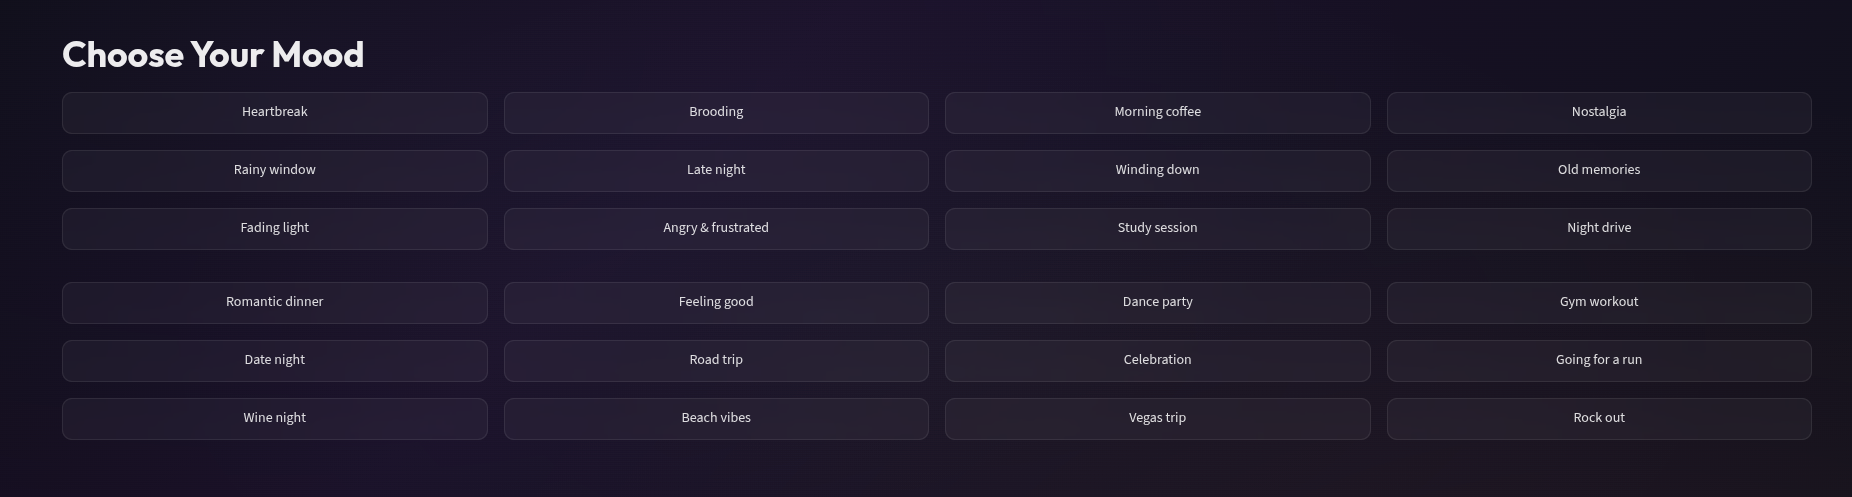
\includegraphics[width=0.95\textwidth]{results/screenshot_presets.png}
\caption{Interfața principală -- selecția preset-urilor de mood}
\label{fig:screenshot_presets}
\end{figure}

\begin{figure}[H]
\centering
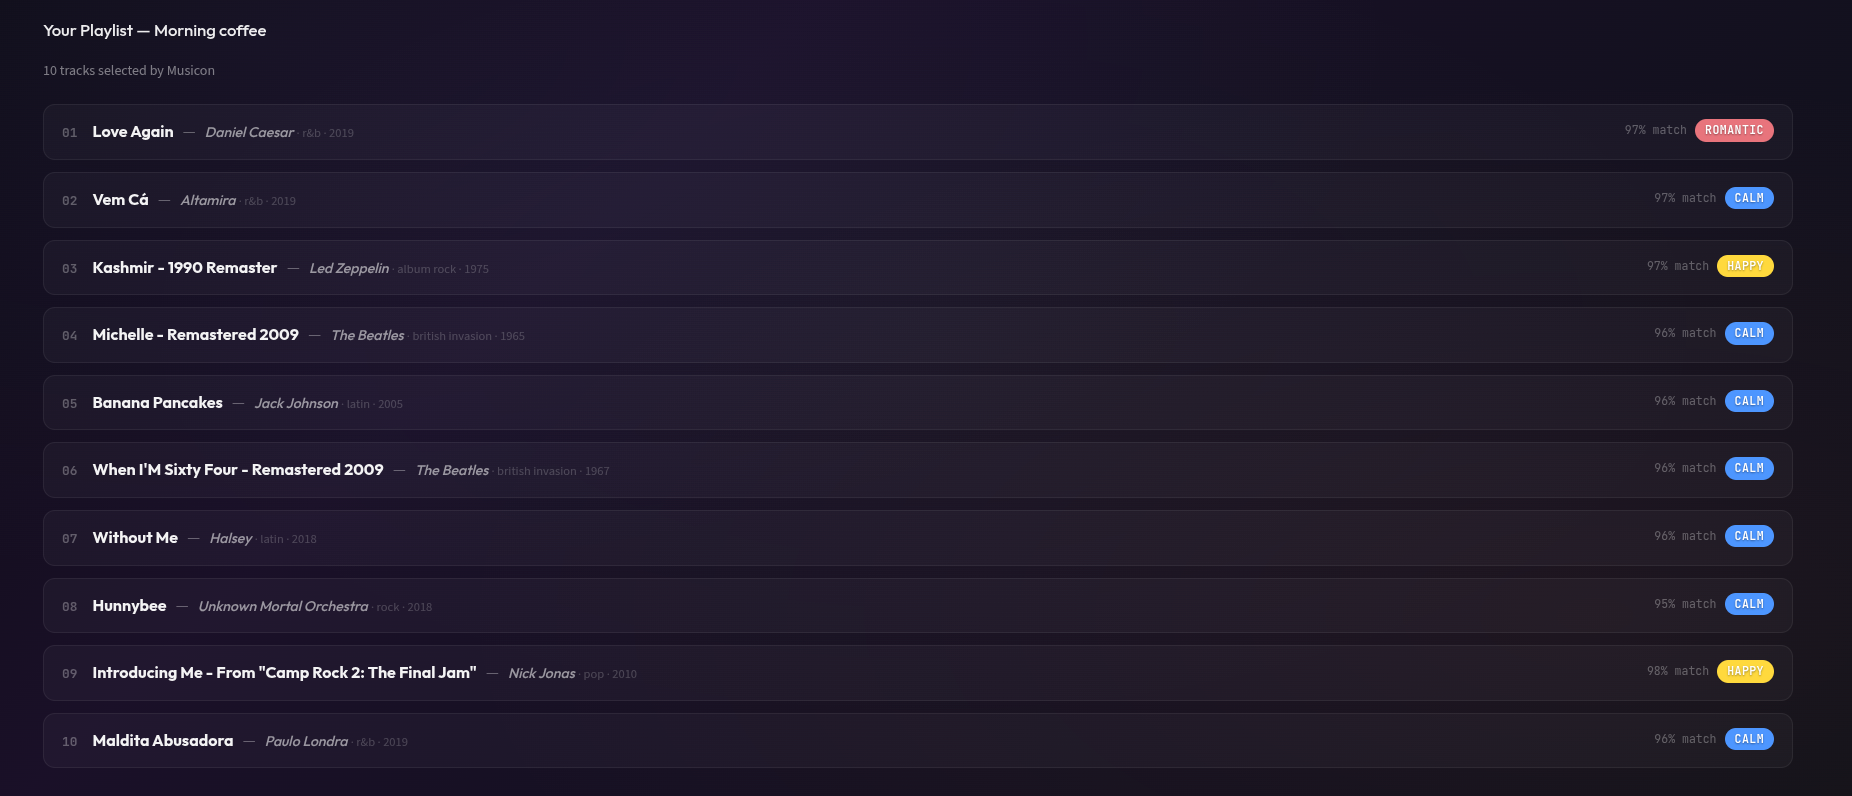
\includegraphics[width=0.95\textwidth]{results/screenshot_playlist.png}
\caption{Playlist generat cu detalii despre piese, similaritate și badge-uri de mood}
\label{fig:screenshot_playlist}
\end{figure}

\begin{figure}[H]
\centering
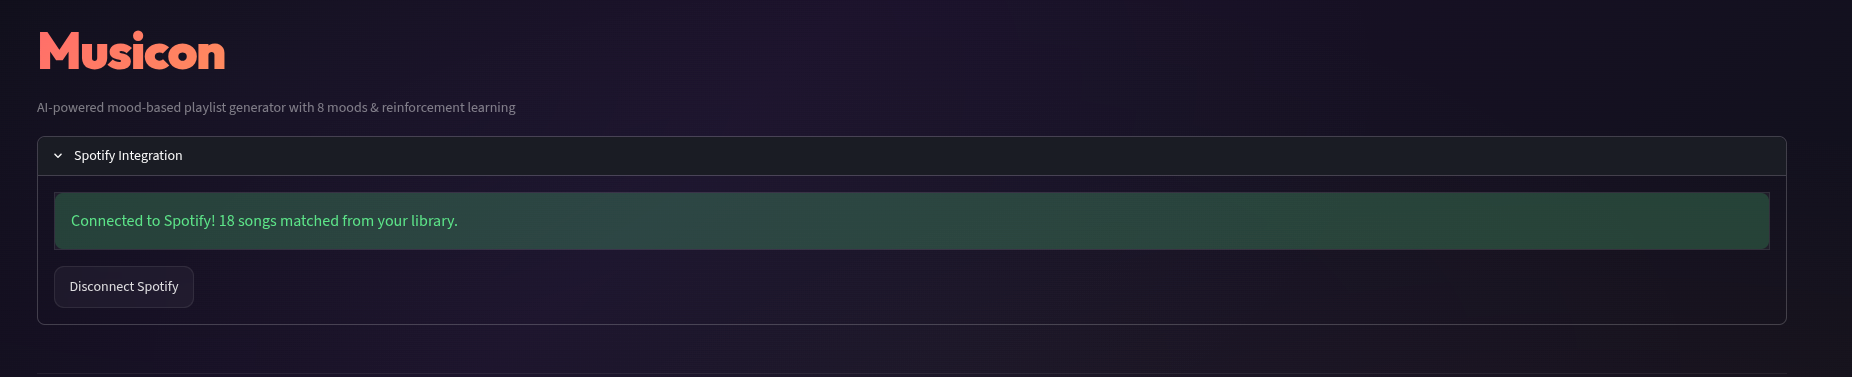
\includegraphics[width=0.95\textwidth]{results/screenshot_spotify.png}
\caption{Integrarea Spotify -- conectarea contului și exportul playlist-ului}
\label{fig:screenshot_spotify}
\end{figure}

\begin{figure}[H]
\centering
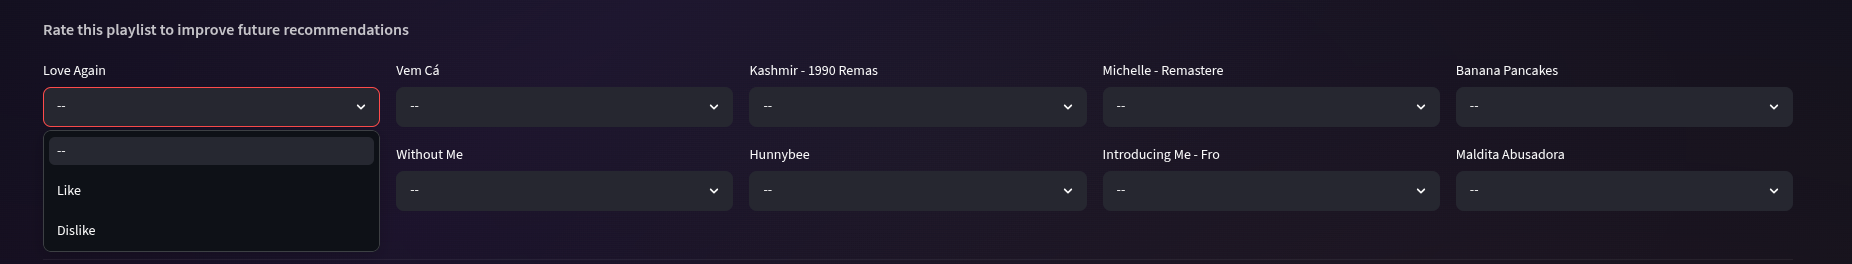
\includegraphics[width=0.95\textwidth]{results/screenshot_feedback.png}
\caption{Mecanismul de feedback Like/Dislike și analiza feature-urilor audio}
\label{fig:screenshot_feedback}
\end{figure}

\begin{figure}[H]
\centering
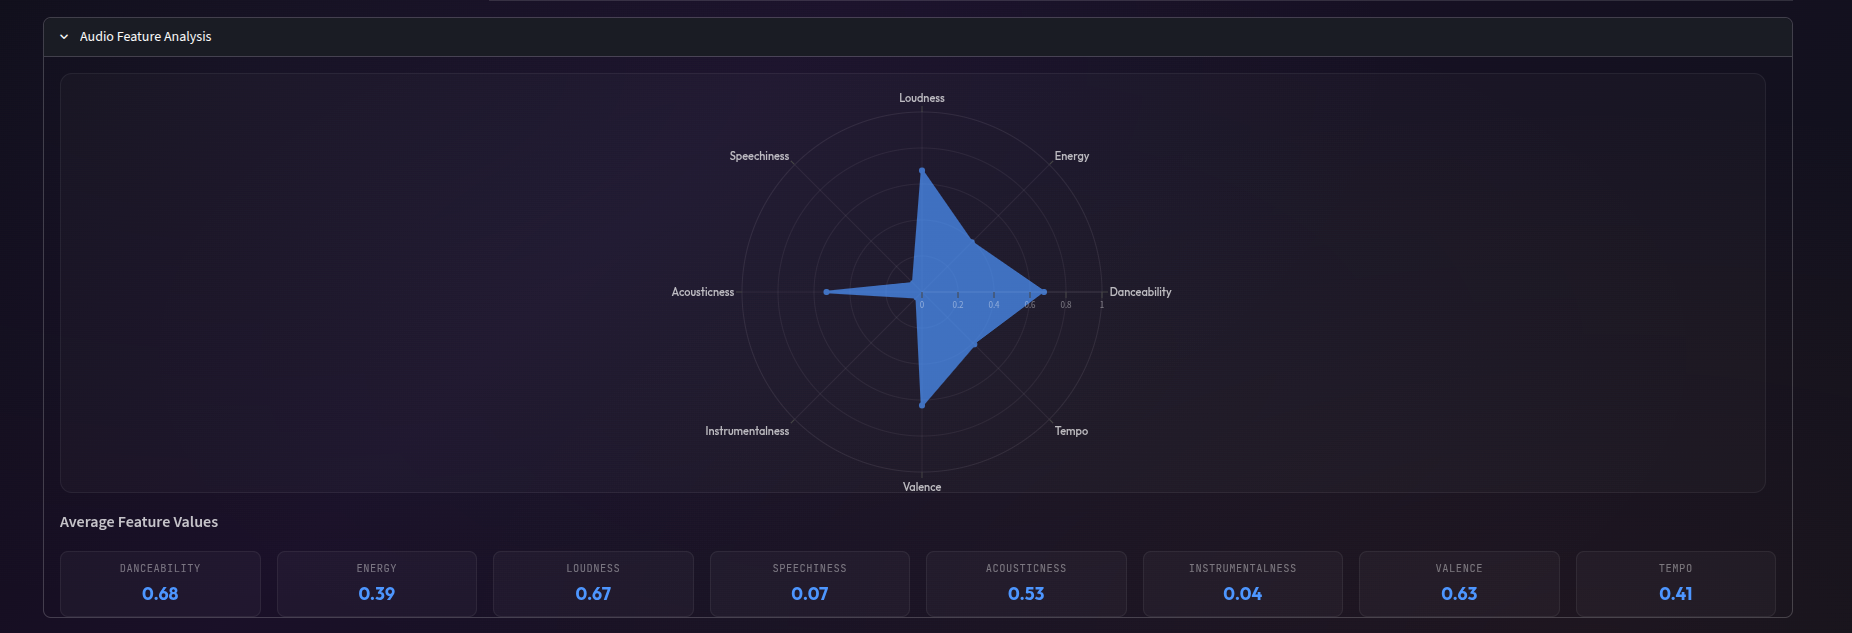
\includegraphics[width=0.7\textwidth]{results/screenshot_radar.png}
\caption{Graficul radar cu profilele audio medii ale playlist-ului generat}
\label{fig:screenshot_radar}
\end{figure}

\end{document}